\label{chap:03_social_text_classification}

La extracción de opiniones en distintos espacios virtuales ha atraído mucho interés desde los comienzos de la Web 2.0. Inicialmente motivados por fines puramente comerciales, diferentes oportunidades han surgido mediante al desarrollo de la técnica y la mayor interacción de usuarios en Internet: desde fines sociológicos --como el análisis de discurso de odio o las reacciones a la pandemia-- hasta políticos -- como observar cuál es la opinión general sobre tal o cual candidato o sobre un tema candente. A partir de los años 2000, y debido a la combinación del desarrollo de métodos de aprendizaje estadístico y la cantidad creciente de datos disponibles generados por usuarios en Internet, numerosos trabajos han analizado este tipo de textos para poder extraer conocimiento \textbf{subjetivo} de quienes vuelcan sus pensamientos en las redes sociales y otros espacios virtuales.

Debido a la inmensa cantidad de contenido generado en diversos sitios y redes sociales (se estima que en el mundo se generan 500 millones tweets por día para 2021\footnote{Fuente: \url{https://www.internetlivestats.com/twitter-statistics/}}), esta tarea es difícil de realizar sin algún tipo de automatización. Para ello, muchísimo esfuerzo se ha volcado en utilizar técnicas de aprendizaje automático para poder extraer este tipo de información de los textos creados por usuarios. El avance de las técnicas de NLP --como hemos descrito en el capítulo anterior-- han permitido avanzar sobre este terreno; sin embargo, muchas de las limitaciones actuales del área junto a las dificultades particulares de las interacciones en medios sociales hacen esta tarea difícil.

En este capítulo haremos una breve introducción al análisis de sentimientos o extracción de opiniones sobre textos de redes sociales. Esto es, dado un texto generado por un usuario (un post en Facebook, Instagram, un tweet, etc) predecir alguna característica discreta de éste, como por ejemplo si es un texto positivo o negativo, si tiene algún tipo de emoción de ira, alegría, u otra; si contiene discurso de odio contra algún grupo o no; si es irónico; entre otras. En base a datasets en español para distintas tareas, presentaremos modelos de clasificación basados en técnicas del estado del arte.

Analizaremos también algunas cuestiones relacionadas a la adaptación de dominio y representaciones generadas sobre dominios de textos generados por usuarios, planteando algunas líneas que retomaremos en capítulos posteriores.


\section{Motivación}

Las motivaciones para extraer opiniones subjetivas de usuarios en Internet son múltiples, aunque intentaremos categorizarlas en algunos grupos de notable interés. Dado el aumento considerable de contenido generado por usuarios desde la popularización de la WWW  --y subsiguientemente con la explosión de las Redes Sociales-- una de las cuestiones que motoriza este área es netamente comercial: ¿qué opinan los usuarios sobre este nuevo producto? ¿cuáles creen que son sus falencias? ¿qué tal es el servicio en tal o cual Restaurant? Desde ya más de 20 años, numerosos sitios y aplicaciones brindan la posibilidad de que los clientes vuelquen sus opiniones al respecto de los productos que consumen en sus plataformas. Para citar unos ejemplos, IMDb permite agregar comentarios sobre películas, Google Maps sobre distintos sitios --tanto turísticos como locales comerciales--, o los distintos sitios de venta minorista como MercadoLibre, eBay, o Amazon sobre los productos que compran sus usuarios. Sobre esta información disponible, una encuesta de 2008 \cite{horrigan2008online} reportó que cerca del 81\% de los usuarios de Internet de entonces (60\% de los habitantes de Estados Unidos) realizaron investigación online antes de sus compras, aunque también reportaban problemas a la hora de encontrar información valiosa para sus fines.

Con la explosión de las redes sociales, nuevas oportunidades y posibilidades de preguntas a contestar se abrieron mediante la extracción de opiniones en este medio \footnote{Si bien algunas preguntas de carácter sociológico tuvieron lugar con anterioridad, podemos marcar el uso intensivo de Facebook y Twitter como el comienzo de un estudio más sistemático de ellas dado el enorme volumen de datos accesibles para los investigadores}. Uno de estos horizontes, que es de interés particular para esta tesis, es el de las preguntas de carácter sociológico y político. Preguntas que pueden suscitar interés dentro de este punto pueden ser:

\begin{itemize}
    \item ¿cuál es la opinión de los usuarios acerca de la legalización del aborto en cierto país que tiene en tratamiento este tema? ¿es representativo de la población en general? \cite{graells2019abortion}
    %\item ¿cuál es el sentimiento que tienen ciertos usuarios hacia los inmigrantes subsaharianos en España?
    \item ¿cómo se ha modificado el humor social de acuerdo a crisis económicas o pandemias como la del COVID-19? \cite{brufau2020emotion}
    \item ¿qué características tiene el discurso de odio  contra los inmigrantes en España en el medio del auge de la ultraderecha en dicho país? \cite{calderon2020topic}
    \item ¿qué artículos periodísticos suscitan la mayor cantidad de discurso discriminatorio en las redes sociales?
    \item ¿cuáles son las principales vulnerabilidades e intereses de ciertos sectores de la población? \cite{zuiderveen2018online} \footnote{Esto, según parece, fue utilizado en el affaire de Cambridge Analytica en las elecciones de 2016 que consagraron a Donald Trump en EEUU}
\end{itemize}

entre otras. Estos tópicos son de gran interés para investigadores y políticos. Usualmente, la forma más estandarizada de acceder a la opinión de distintos actores sociales ha sido la de encuestas; sin embargo, la recolección y extracción automática de opiniones de medios virtuales brinda una alternativa (a veces) más económica y masiva aunque con un sesgo poblacional distinto al de otras metodologías.

\section{Clasificación de textos sociales}

Muchos de estos problemas de extracción de opiniones se pueden plantear como tareas de clasificación de texto \cite{pang2008opinion}. El análisis de polaridad se puede plantear como una tarea de predecir si un texto tiene un sentimiento positivo, negativo, o neutro. El análisis de emociones se puede plantear (entre otras formas) como la de predecir la emoción predominante en el texto sobre un conjunto de seis posibles emociones.

Algunas variantes de estos problemas se pueden dar en el contenido analizado. El \emph{Análisis de Sentimiento basado en aspectos} (usualmente denominada \emph{ABSA} en la literatura por sus siglas en inglés) es una variante de la clasificación de polaridad en la que queremos predecir el sentimiento de un texto para cierto aspecto \cite{pavlopoulos2014aspect}; por ejemplo, en la oración ``lindo lugar, la comida está muy bien pero la cerveza es horrible'' (en una posible reseña de un restaurant) podemos identificar dos sentimientos distintos: uno positivo para la comida y otro negativo para la cerveza. Dentro de estos problemas que complejizan la entrada, podemos contar algunos de carácter multimodal: en \citet{sharma-etal-2020-semeval} se plantea un problema de análisis de emociones para memes donde la entrada (el contenido social) consta de imágenes y texto, y se intenta predecir la emoción predominante.

Análogamente, se puede agregar cierta complejidad en la salida. El \emph{Stanford Sentiment Treebank (SST)} \cite{socher-etal-2013-recursive} plantea una tarea de análisis de polaridad asignando una escala de Likert \cite{likert1932technique} donde cada comentario está etiquetado como muy negativo, algo negativo, neutral, algo positivo o muy positivo. Así mismo, otra posibilidad es la de predecir conjuntamente varias variables: por ejemplo, predecir si un comentario es discriminatorio, si es dirigido a un grupo o una persona, y si es agresivo, como el dataset de hatEval \cite{hateval2019semeval}; o bien, dado un comentario de una nota periodística, predecir las características que discrimina si es que hay alguna (como ser a las mujeres, al colectivo LGBTI, por motivos raciales, etc). De este último ejemplo hablaremos en los capítulos \ref{chap:05_dataset_creation} y \ref{chap:06_contextualized_hate_speech}.


\section{Trabajo previo}

El análisis de sentimientos, opinion mining u opinion extraction suscitó interés casi desde el comienzo de la generación masiva de contenido de parte de los usuarios en la WWW. Particularmente desde la eclosión de las redes sociales, la inmensa cantidad de contenido generado por usuarios ha sido una fuente de información sin antecedentes para la extracción de todo tipo de opiniones. La bibliografía que comprende este tema es demasiado extensa y escapa los objetivos de esta tesis centrada en la detección de discurso de odio. Mencionamos algunos estudios exhaustivos relevantes y una pequeña selección de trabajos a continuación.

\citet{pang2008opinion} ofrecen un amplio repaso sobre los usos, aplicaciones, técnicas y dificultades de la extracción de opiniones en la era pre-deep learning y pre-redes sociales, mencionando cuestiones como las dificultades que los diferentes dominios presentan a las técnicas del entonces estado del arte. El trabajo de \citet{pak2010twitter} es uno de los pioneros en plantear a Twitter como una fuente de mensajes para la extracción de opiniones -- en particular, para analizar polaridad de mensajes -- proponiendo una metodología para recolectar y etiquetar datasets sobre esta red social. \citet{yue2019survey} presentan un racconto de los diversas tareas de análisis de sentimientos aplicados a textos de redes sociales y las técnicas para atacarlo.

Dentro de los recursos para tareas de opinion mining, \citet{maas-EtAl:2011:ACL-HLT2011} presenta un dataset de análisis de polaridad con dos etiquetas (positivo y negativo) sobre películas en la plataforma de IMDb, extensamente utilizado para la tarea de análisis de sentimientos. El Stanford Sentiment Treebank (SST) \cite{socher-etal-2013-recursive} es un dataset que contiene información granular en una escala símil Likert de polaridad sobre las distintas subpartes de cada oración. Esta tarea forma parte del benchmark de General Language Understanding Evaluation (GLUE) \cite{wang-etal-2018-glue}. El workshop SemEval \footnote{\url{https://semeval.github.io/}} ha generado numerosos recursos para tareas de opinion mining en redes sociales, como Análisis de Polaridad, Análisis de Polaridad basado en aspectos, análisis de emociones, entre otras.

Centrándonos en los recursos y tareas en español, uno de los principales polos de esto es el Taller de Análisis de Sentimientos (TASS) \cite{overview_tass2018,garcia2020overview,cumbreras2016overview} organizado por la Sociedad Española de Procesamiento Natural (SEPLN) y a partir de 2020 en el marco del evento Iberian Languages Evaluation Forum (IberLEF). En este foro se presentaron tareas y datasets de análisis de sentimiento \cite{garcia2020overview}, de emociones \cite{plaza-del-arco-etal-2020-emoevent}, de toxicidad \cite{taule2021detoxis}, entre otras.


\section{Tareas analizadas}
\large
\begin{table}[t]
    \centering
    \begin{tabular}{ p{0.30\textwidth}  p{0.15\textwidth} p{0.15\textwidth} p{0.15\textwidth} p{0.1\textwidth}}
        \hline
        Tarea                     &  Dataset                   & \#Mensajes     & Clases   &\\
        \hline
        \mr{3}{Análisis de Sentimientos}  &  \mr{3}{TASS 2020} & \mr{3}{$14,509$} & Neg      & (39.8\%)\\
                                          &                    &                & Neu      & (29.5\%)\\
                                          &                    &                & Pos      & (30.7\%)\\
        \hline
        \mr{7}{Análisis de Emociones}&\mr{7}{EmoEvent}&\mr{7}{$8,409$}  & Otra    & (49.08\%)  \\
                                          &                    &                & Alegría  & (21.6\%)  \\
                                          &                    &                & Tristeza & (12.0\%)  \\
                                          &                    &                & Ira      & (10.2\%)  \\
                                          &                    &                & Sorpresa & (4.1\%)  \\
                                          &                    &                & Disgusto & (1.9\%)  \\
                                          &                    &                & Miedo    & (1.1\%)  \\
        \hline
        \mr{2}{Detección de Ironía}  & \mr{2}{IroSVa 2019}     & \mr{2}{$9,000$}  & No irónico   & (66.7\%)\\
                                          &                    &                & Irónico      & (33.3\%)\\
        %Análisis de Emociones     &  TASS 2020/EmoEvent\cite{plaza-del-arco-etal-2020-emoevent} & 7 & 1,879 \\
        \hline
    \end{tabular}
    \caption{Tareas evaluadas en este capítulo, junto a datos estadísticos de los datasets utilizados}
    \label{tab:03_tasks}
\end{table}

Tres tareas de extracción de opiniones sobre redes sociales fueron utilizadas como benchmark para las diferentes técnicas de clasificación. La Tabla \ref{tab:03_tasks} contiene información sobre las tareas analizadas y los datasets utilizados para ellas. Una de las tareas es la de \textbf{análisis de polaridad}: dado un tweet, detectar si tiene una polaridad general positiva, negativa, o neutra. Utilizamos el dataset de TASS 2020 \cite{garcia2020overview}, anotado con estas 3 clases y con información de las diferentes variedades dialectales del español a la que pertenece cada tweet. Para nuestro análisis, ignoramos estas distinciones y fusionamos todos los datos en un solo conjunto de datos (con las tres particiones correspondientes de entrenamiento, validación, y test).

Para el \tbf{análisis de emociones}, también usamos el conjunto de datos de TASS 2020 \emph{EmoEvent} \cite{plaza-del-arco-etal-2020-emoevent}. Este dataset multilingual (español e inglés) contiene tweets etiquetados con las seis emociones básicas de Ekman :\emph {ira}, \emph {disgusto}, \emph {miedo}, \emph {alegría}, \emph {tristeza}, \emph {sorpresa} y también una emoción \emph{neutral} \cite{ekman1992argument}. El dataset fue recolectado en base a a ocho eventos globales de diferentes dominios (políticos, entretenimiento, catástrofes o incidentes, conmemoraciones globales, etc.) por lo que las emociones siempre están relacionadas con un fenómeno en particular. Solo conservamos la parte en español, que contiene $8,409$ tweets.


 La \textbf{detección de ironía} es una tarea que ha ganado popularidad recientemente. Algunos trabajos han mostrado que tiene importantes implicaciones en otras tareas de NLP de caracter semántico: para citar uno, \citet{gupta-yang-2017-crystalnest} muestran que el uso de funciones derivadas de la detección de sarcasmo mejora el rendimiento de ciertos modelos en la tarea de análisis de sentimientos. Además de esto, el contenido generado por los usuarios es una rica y vasta fuente de ironía, por lo que esta tarea es de particular importancia para el dominio de las redes sociales. IroSVa \cite {ortega2019overview} es un dataset en Español (publicado en el contexto de TASS 2019) que tiene la particularidad de considerar los mensajes no como textos aislados sino con un contexto dado (un titular o un tema). Consta de $7,200$ instancias y $1,800$ ejemplos de prueba divididos en tres variantes geográficas de Cuba, España y México, cada una con una etiqueta binaria que indica si el comentario contiene ironía o no. A diferencia de las dos tareas anteriores mencionadas aquí, este conjunto de datos contiene no solo mensajes de Twitter, sino también de comentarios de noticias y foros de debate como 4forums.com y Reddit.

 La Tabla \ref{tab:03_datasets_examples} ilustra algunos ejemplos seleccionados para las distintas tareas y sus clases. En el caso de la tarea de detección de emociones, podemos ver que algunos ejemplos han sido preprocesados por sus autores para ocultar los hashtags y urls.

\begin{table}
    \centering
    \begin{tabularx}{\textwidth}{l l X}
        Tarea                          & Clase        & Ejemplos         \\
        \Xhline{4\arrayrulewidth}
\rule{0pt}{4ex}\mr{7}{Emociones}       & Neutral        & Espectantes para ver el tercer capitulo de HASHTAG. El principio empieza bien.	\\
                                       & Alegría        & Lo de Messi ha sido increíble! HASHTAG        \\
                                       & Tristeza       & Un día lamentable. Se perdieron años de historia, de cultura, de arquitectura... Me siento devastada al ver las imágenes del incendio de la catedral de HASHTAG en HASHTAG URL \\
                                       & Ira            & URL que discurso para ponerlo a llorar, Putos humanos, para cuando la extinción?? \\
                                       & Sorpresa       & Santa Maria Madre de Dios HASHTAG URL \\
                                       & Miedo          & Joder, izquierda venció ¿y qué? A mi me preocupa y mucho que Vox haya pasado de 0 a 24!! ¿a nadie le parece un montón? No sé, debo ser idiota. HASHTAG	\\
                                       & Disgusto       & Como se nota que HASHTAG ya no tiene el apoyo de los libros. Vaya mierda de temporada se están sacando.	 \\
        \hline
\rule{0pt}{4ex}\mr{3}{Sentimientos}    & Negativo       & que triste es la realidad	\\
                                       & Positivo       & Hola a todos corazones, buen día Y FELIZ NAVIDAD A TODOS USTEDES! DIOS ME LOS BENDIGA Y ME LOS LLENE DE TODO SU AMOR \\
                                       & Neutral        & $@$AlfonsoEmilioL La próxima vez que no vea lo entrevisto y pregunto que escucha.	\\
        \hline

\rule{0pt}{4ex}\mr{4}{Ironía}          &\mr{3}{Irónico} & Pues, noticia de última hora, eres un anormal que no sabe escribir. Es LESIONARAN.    \\
                                       &                & El juez paraliza la exhumación de Franco alegando peligro para los operarios. Pues me parece muy bien, porque con las ratas hay que ser muy precavido.	\\

                        \rule{0pt}{2ex}& No irónico     & No me sirvió para nada todo fue en vano. Espero mejore la calidad.	\\
        \Xhline{4\arrayrulewidth}
    \end{tabularx}
    \caption{Ejemplos de instancias para las distintas tareas y clases.}
    \label{tab:03_datasets_examples}
\end{table}



\section{Normalización y preprocesamiento}
\label{sec:03_preprocessing}

Una de los pasos más importantes para la manipulación de texto proveniente de redes sociales es el preprocesamiento. Con esto nos referimos al conjunto de técnicas dedicadas a disminuir la variabilidad del texto y aproximarlo a una forma lo más normal posible, aún cuando ciertos autores discuten la existencia de tal forma \cite{eisenstein2013bad}. El texto generado por usuarios en medios informales suele ser más irregular que el texto proveniente de otras fuentes, con errores ortográficos, usos coloquiales y otros usos que hacen difícil el tratamiento por algoritmos de NLP. Para poner un ejemplo, la frase ``¡qué lindo día, loco!'' puede ser representada de las siguientes maneras:

\begin{itemize}
    \item q lindo día loco
    \item k lindo diaaaaaaaa loco
    \item ke lendo diaa lk
\end{itemize}

\noindent entre otras formas posibles. Uno de los primeros trabajos que aborda este problema para el dominio de redes sociales es el de \citet{han2011lexical}. En base a un dataset de tweets, observaron que las palabras fuera de vocabulario (OOV en inglés) \footnote{fuera del vocabulario de un diccionario estándar de GNU en inglés} en dicha red social tienen una alta frecuencia de incidencia. Ejemplos de estas palabras son neologismos, errores ortográficos, typos, contracciones típicas de esta red social (lk), sustituciones fonéticas (wacho en vez de guacho), entre otras. Este problema de la desnormalización del texto generado por usuarios planteaba un serio inconveniente para los métodos del estado del arte de ese entonces basados en bolsas de palabras o representaciones sobre palabras aisladas \footnote{Recordemos que para el momento de la publicación de este trabajo aún no se usaban redes neuronales, word embeddings, ni mucho menos métodos más avanzados como \emph{fasttext}, que ayuda mucho en las palabras OOV}. Para mitigar la alta dimensionalidad que generan estas palabras fuera de vocabulario, los autores propusieron diversas estrategias para normalizar las palabras y testean sus métodos sobre datasets de Twitter y SMS.

El trabajo de \citet{eisenstein2013bad} trató desde una perspectiva más amplia los enfoques utilizados hasta el momento para tareas en medios sociales, planteando dos posibilidades: la \textbf{normalización} sería una forma de adaptar el texto a las herramientas, mientras que la \textbf{adaptación de dominio} sería adaptar las herramientas al texto. Con lo primero, el trabajo menciona al conjunto de técnicas que podemos utilizar para acercar la distribución del texto lo más posible a un dominio formal, mientras que por adaptación de dominio a la construcción de conjuntos de datos y algoritmos particulares para distintas tareas de NLP en redes sociales, como por ejemplo POS tagging \cite{gimpel2010part}, NER \cite{ritter2011named}, entre otros.


La alta desnormalización siguió siendo un escollo para los modelos basados en redes neuronales y embeddings (como \emph{GloVe} o \emph{word2vec}) ya que cada representación se calcula sobre las palabras o tokens de la oración. En el caso de un elemento fuera de vocabulario, un mecanismo habitual es asignarles un token especial ``<unk>'', y por lo tanto, una única representación para todas esas palabras OOV. Sin embargo, esto puede ser problemático ya que elimina muchas palabras similares a otras que sí tenemos en el vocabulario. \citet{bojanowski16} propuso una solución a esto al permitir formar la representación de cada palabra mediante una combinación lineal de las representaciones de las ``subpalabras'' de cada una (ver Sección \ref{sec:02_representaciones}).

Con el advenimiento de los modelos basados en transformers, otros tipos de tokenización fueron propuestos que permiten reducir las palabras OOV. Word Piece \cite{schuster2012japanese} y Sentence Piece \cite{kudo-richardson-2018-sentencepiece} son algoritmos de tokenización que, en lugar de partir la palabra en tokens o n-gramas de caracteres fijos como \emph{fasttext}, convierten cada palabra en una tira de subpalabras provenientes de un vocabulario. Estos vocabularios no están prefijados sino que son entrenados sobre conjuntos de datos con variantes de Byte-Pair Encoding (BPE) \cite{sennrich2016neural} que intentan minimizar la cantidad de tokens utilizados para representar el texto. Esta técnica permite reducir la incidencia OOV notablemente, ya que muchas de estas subpalabras entrenadas guardan relación morfológica con el idioma (y el dominio) de los datos de entrenamiento.

\citet{dat2020bertweet} plantearon experimentos en tareas sobre texto proveniente de redes sociales usando dos formas de normalización: una \textbf{débil}, donde sólo convirtieron nombres de usuario en un token especial \verb|@USER| y a las URLs en otro token especial \verb|HTTPURL|, y otra estrategia \textbf{fuerte} donde utilizaron diccionarios de normalización y otras técnicas para reducir la variabilidad del texto basadas en \citet{han2011lexical}. Para un conjunto de tareas de clasificación sobre Twitter y distintos modelos pre-entrenados, los resultados de los experimentos arrojaron que la normalización fuerte empeora levemente la performance.

Teniendo estas consideraciones en cuenta, adoptamos una estrategia similar a la normalización \textbf{débil} mencionada en el trabajo recién mencionado:

\begin{itemize}
    \item Convertimos los handles a un token especial \verb|@usuario|
    \item Convertimos las URLs a un token especial \verb|URL|
    \item Convertimos los emojis a representaciones textuales usando la librería \emph{emoji} \footnote{\url{https://pypi.org/project/emoji/}}
    \item Normalizamos risas (``jajajajjjjajaja'' lo convertimos a ``jaja'')
    \item Procesamos hashtags: \#EsteHayQueNormalizar lo convertimos a \emph{hashtag esto hay que normalizar}, utilizando las mayúsculas dentro del hashtag
    \item Limitamos repeticiones de caracteres a 3 ocurrencias
\end{itemize}

Si bien en algunos fragmentos de esta tesis usamos variaciones de estos métodos (como por ejemplo en la Sección \ref{sec:04_preprocessing}), en general seguiremos esta estrategia de normalización.

\section{Modelos de clasificación}
\label{sec:03_classification}

\begin{figure}
    \centering
    % Link a draw
    % https://docs.google.com/drawings/d/1bSCMXkAF12gK4GFYL8tyIAPCMq4kj8JXovrf2lx5w_g/edit
    \begin{subfigure}[t]{\textwidth}
        \centering
        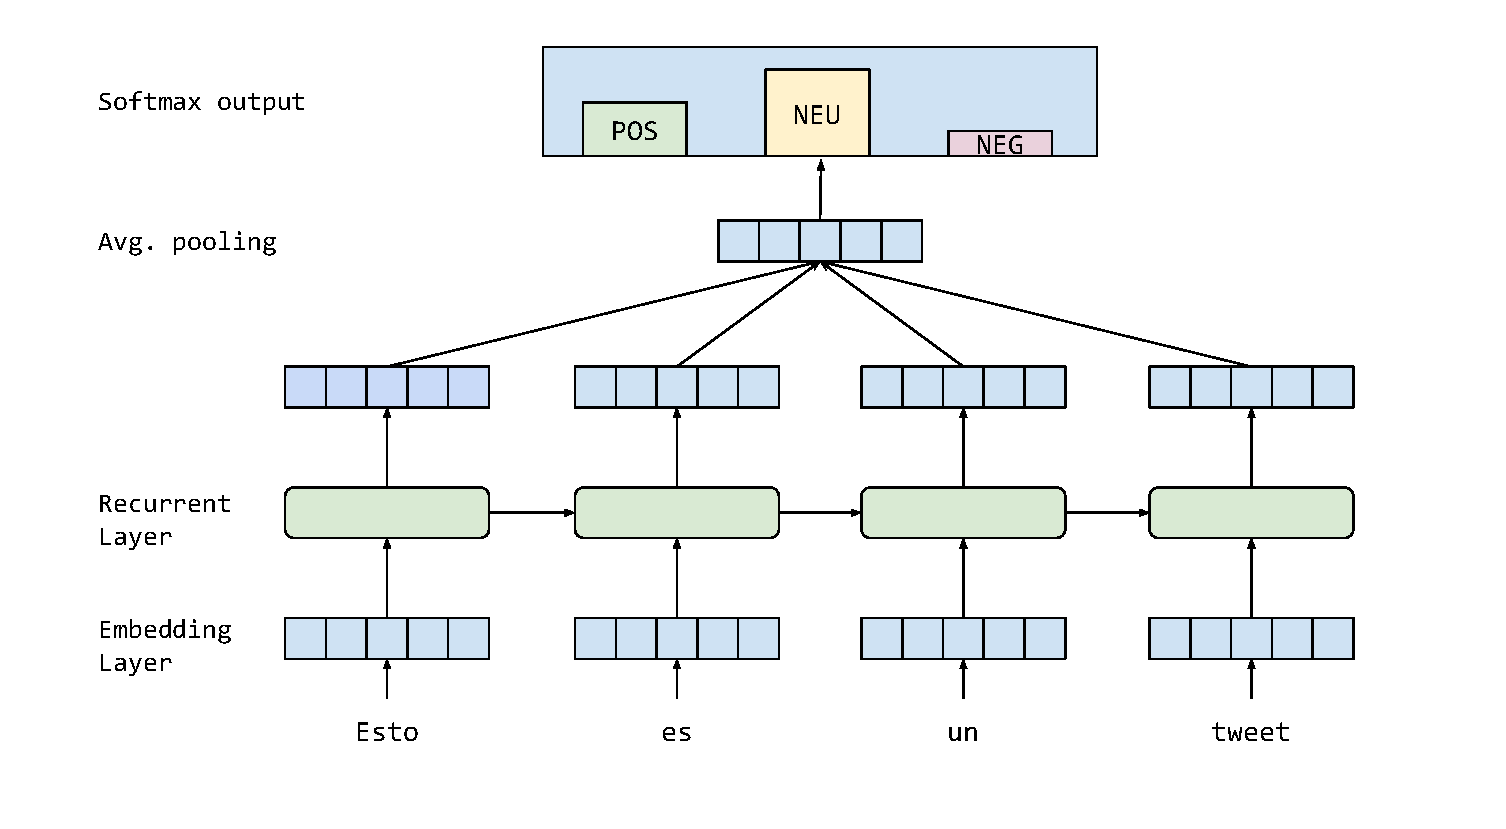
\includegraphics[width=\textwidth]{img/03/recurrent_classifier.pdf}
        \caption{Clasificador basado en redes recurrentes}
        \label{subfig:rnn_classifier}
    \end{subfigure}
    % Link a draw
    % https://docs.google.com/drawings/d/1KWz2NJGVoTO-pAAhhLjoX4AT-kSbK3yapLKLuQ2E9zw/edit
    \begin{subfigure}[t]{\textwidth}
        \centering
        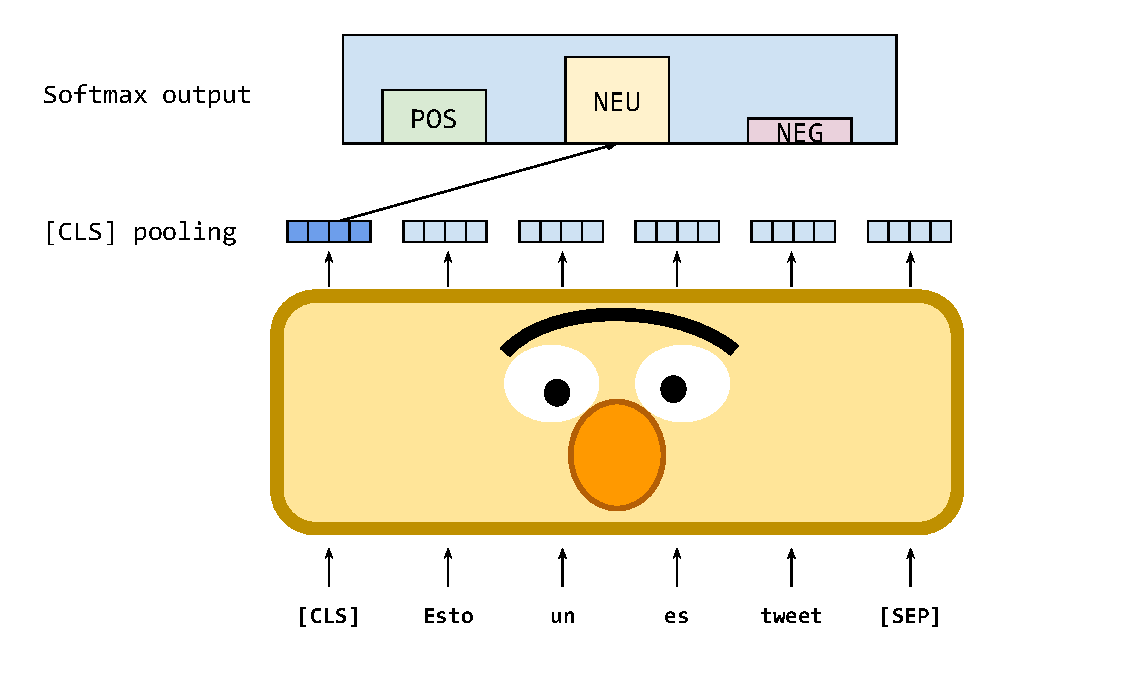
\includegraphics[width=\textwidth]{img/03/bert_classifier.pdf}
        \caption{Modelos de clasificación basado en BERT y símiles}
        \label{subfig:bert_classifier}
    \end{subfigure}

    \caption{Clasificadores propuestos para las tareas de Análisis de Polaridad, Análisis de Emociones y Detección de Ironía. La subfigura \ref{subfig:rnn_classifier} muestra la arquitectura del modelo recurrente, que usa una capa de embeddings basados en \emph{fasttext} y codifica el tweet como el promedio de las salidas de la capa recurrente. La subfigura \ref{subfig:bert_classifier} muestra un clasificador basado en BERT, donde tomamos la salida del token \clstok{} como la codificación del tweet. Ambos usan un decodificador softmax}
    \label{fig:03_classifiers}
\end{figure}

Describimos a continuación los clasificadores utilizados para las tareas. Podemos, a grandes rasgos, describir a todos nuestros clasificadores como compuestos de dos partes: un \emph{codificador} (o \emph{encoder} en inglés) que genera una representación continua de longitud fija del texto de entrada, y un \emph{decodificador} que toma esa codificación y la convierte a la salida deseada.

Todos nuestros problemas son de clasificación múltiple: elegir exactamente una clase entre varias. Para ello, nuestro decodificador será de la forma $\softmax(Wx + b)$, donde $W \in \mathbb{R}^{c \times h}$ es una matriz de pesos y $b \in \mathbb{R}^c$ un vector de sesgo, siendo $c$ la cantidad de clases y $h$ el tamaño de la codificación de entrada. Los clasificadores planteados difieren entonces en los codificadores. Propusimos las siguientes variantes:

\begin{itemize}
    \item \textbf{FFN}: un perceptrón multicapa (feed-forward network) con una función de activación intermedia \emph{ReLU}
    \item \textbf{GRU/biGRU}: una red neuronal recurrente donde la capa oculta es una Gated Recurrent Unit (GRU) unidireccional o bidireccional.
    \item \textbf{Transformers}: un modelo pre-entrenado de lenguaje basado en transformers. Consideramos los modelos \beto{} \cite{canete2020spanish}, \roberta{} en su versión en español \cite{gutierrezfandino2021spanish}, \emph{BERTin} \footnote{\url{https://huggingface.co/bertin-project/bertin-roberta-base-spanish}}, como así también el modelo multilingual \emph{mBERT}
\end{itemize}

La capa de entrada de los modelos \textbf{FFN} y \textbf{GRU/biGRU} fueron entrenados con embeddings no contextualizados basados en \fasttext{}. Utilizamos dos versiones de estas representaciones: las canónicas generadas por los autores, entrenadas sobre Common Crawl en español; y también una versión generada por nosotros, entrenada sobre tweets en español, cuya recolección describimos en la Sección \ref{sec:robertuito_data_collection}.

La codificación final que utilizamos para la red \textbf{GRU/biGRU} se da como el promedio de los vectores salida de cada paso. Para los modelos basados en transformers, la codificación se da tomando la salida del caracter de inicio (\clstok{}). Si bien podría también tomarse el promedio como en las redes recurrentes, los modelos basados en transformers no sufren el cuello de botella que se genera tomando la última representación de la red recurrente. La Figura \ref{fig:03_classifiers} ilustra la arquitectura de los clasificadores recurrentes y basados en transformers.


Usamos un tamaño oculto de 512 para los modelos exceptuando los basados en Transformers --que suelen tener $768$ como valor estándar-- y para todos los casos una regularización del tipo dropout \cite{srivastava2014dropout} de $0.1$ sobre la codificación del tweet. Como algoritmo de optimización utilizamos \emph{Adam} \cite{kingma2014adam} con un learning rate de $0.001$ y un decay de $0.01$. Para los clasificadores basados en transformers, usamos Adam con un learning rate triangular de $10^{-5}$ y un warmup del 10\% de los pasos. Entrenamos todos los modelos por 5 epochs y nos quedamos con los modelos que mejor performance tengan sobre el split de validación en términos de la métrica correspondiente a la tarea.


\section{Resultados}

\begin{table*}[t]
    \centering
    \large
    \begin{tabular}{l ccc l}
        \toprule
        Modelo         &  Polaridad         & Emociones         &   Ironía        &  Puntaje \\
        \hline
        RoBERTa        &  $67.0 \pm 0.6$ &  $52.7 \pm 1.5$ & $72.1 \pm 0.8$ & $66.46$ \\
        BERTin         &  $66.6 \pm 0.5$ &  $52.4 \pm 0.7$ & $71.3 \pm 1.2$ & $66.01$ \\
        BETO$_U$       &  $65.1 \pm 0.6$ &  $53.2 \pm 1.2$ & $70.1 \pm 0.7$ & $65.26$ \\
        BETO$_C$       &  $66.2 \pm 0.5$ &  $51.6 \pm 1.2$ & $70.5 \pm 0.9$ & $65.17$ \\
        mBERT          &  $61.7 \pm 0.3$ &  $49.3 \pm 1.0$ & $68.1 \pm 1.0$ & $62.73$ \\
        \hline
        biGRU$_{TW}$   &  $58.5 \pm 1.1$ &  $26.4 \pm 0.7$ & $63.1 \pm 1.1$ & $51.80$ \\
        biGRU$_{CC}$   &  $60.2 \pm 0.4$ &  $26.9 \pm 0.3$ & $62.8 \pm 1.4$ & $50.94$ \\
        GRU$_{TW}$     &  $55.3 \pm 0.8$ &  $23.1 \pm 0.6$ & $62.5 \pm 0.9$ & $48.57$ \\
        GRU$_{CC}$     &  $56.4 \pm 0.4$ &  $23.7 \pm 0.5$ & $58.1 \pm 1.6$ & $47.44$ \\
        FFN$_{TW}$     &  $53.8 \pm 0.5$ &  $20.2 \pm 0.2$ & $57.9 \pm 1.2$ & $44.05$ \\
        FFN$_{CC}$     &  $51.1 \pm 0.3$ &  $17.3 \pm 0.2$ & $51.1 \pm 0.5$ & $39.67$ \\

        %robertuito     &  0.560 \pm 0.010 &  0.759 \pm 0.007 &  0.739 \pm 0.005 &  0.705 \pm 0.003 &  0.691 \\
        \hline
    \end{tabular}
    \caption{Resultados de la evaluación de los distintos modelos para las tareas analizadas (Análisis de Emociones, Análisis de Emociones, Detección de Ironía). Los resultados están dados en porcentajes de Macro F1, y expresados como la media de diez corridas junto a su desviación estándar. El puntaje de cada modelo es el promedio de las métricas para las tres tareas}
    \label{tab:03_classification_results}
\end{table*}

La Tabla \ref{tab:03_classification_results} muestra los resultados obtenidos por los distintos modelos, expresados como la media de diez corridas de los experimentos de clasificación junto a sus desviaciones estándar. A su vez, reportamos un puntaje promedio entre todas las tareas. Puede observarse que los modelos basados de transformers obtienen un rendimiento sustancialmente mejor que los basados en redes neuronales recurrentes. Entre los primeros, la versión española de \roberta{} obtiene marginalmente los mejores resultados.

Dentro de los clasificadores de redes recurrentes y feed-forward, aquellos que consumen embeddings entrenados en textos sociales (marcadas como $_{TW}$) tienen un rendimiento superior que aquellos que consumen embeddings entrenados en Common Crawl (marcados como $_{CC}$). Esta diferencia, en todos los casos, es estadísticamente significativa luego de realizar un test de Mann-Whitney U ($p \leq 0.05$ para el caso de ironía y \emph{biGRU}, para todas las demás comparaciones $p \leq 0.001$).



\section{Discusión}

Para las 3 tareas planteadas, los clasificadores basados en modelos pre-entrenados de transformers obtuvieron mejores resultados que los basados en redes recurrentes y feed-forward. Como es esperable (y se observa en la literatura) los modelos monolinguales (\roberta{}, BERTin y \beto{}) tienen un rendimiento sensiblemente mejor el modelo multilingual \emph{mBERT}. Dentro de los modelos de mejor performance se posiciona primero \roberta{}, aunque su mejora es pequeña respecto de \beto{}.

Algo que observamos es que, entre los modelos recurrentes y feed-forward que consumen word-embeddings, la utilización de representaciones entrenadas directamente sobre textos generados por usuarios resultan en una mejor performance de los clasificadores sobre estas tareas que tienen datos de ese mismo dominio. Si bien puede pensarse que el entorno pequeño o el texto ruidoso de los textos pueden ser un problema a la hora de construir representaciones, los experimentos realizados indican lo contrario. Retomaremos esta idea en el Capítulo \ref{chap:07_domain_adaptation}, donde por un lado generaremos un modelo basado en \roberta{} entrenado sobre tweets, y por otro lado observaremos si podemos replicar su performance intentando adaptar un modelo \beto{} a este nuevo dominio.

% Finalmente, como un pequeño aporte -- principalmente a la comunidad académica, y puntualmente aquella hispanoparlante -- creamos una librería de análisis de sentimientos \textbf{pysentimiento} que provee modelos pre-entrenados y herramientas de preprocesado para textos sociales. En esta herramienta quedarán volcados todos los modelos entrenados de esta tesis.

\newcommand{\pysentimiento}[0]{\textbf{pysentimiento}}
\section{\pysentimiento: un paquete de python para Análisis de Sentimiento}


Algo que suele obstaculizar la utilización de herramientas de extracción de opiniones en redes sociales con fines de investigación es la dificultad a su acceso. O bien estos servicios están detrás de sistemas privados detrás de APIs con precios demasiado altos para los presupuestos académicos o están disponibles pero no en español u otros idiomas de bajos recursos \footnote{La definición de bajos recursos es subjetiva, pero tomando en cuenta la cantidad de hablantes nativos de español hay una desproporción abismal con otros idiomas}. En otros casos, estos recursos están disponibles pero no para ser usados de manera sencilla, lo cual es un escollo para investigadores que no sean expertos en NLP.

Como una pequeña contribución de esta tesis y con el objetivo de facilitar el acceso de estos recursos para la investigación, creamos el paquete \textbf{pysentimiento} \footnote{\url{https://github.com/pysentimiento/pysentimiento}}. Esta biblioteca provee modelos pre-entrenados y herramientas de preprocesado para textos sociales en español e inglés. Si bien tiene soporte multilingual, su eje es el de proveer recursos para el español que tiene una disparidad importante en recursos.

\pysentimiento{} utiliza el model hub de \emph{huggingface} \footnote{\url{https://huggingface.co/models}}, un repositorio de modelos de libre acceso. Allí es donde alojamos todos los modelos entrenados, tanto de sentimientos, emociones, y algunos más que serán discutidos a lo largo de esta tesis. Cada tweet que es analizado por la librería pasa primero por una etapa de preprocesamiento (siguiendo el proceso explicado en la Sección \ref{sec:03_preprocessing}), y luego analizado por el modelo que nos brinda la salida correspondiente.

Al momento de escribir estas líneas, los modelos de \pysentimiento{} se encuentran entre los más descargados de \emph{huggingface} para el idioma español, dando cuenta de la necesidad de estas herramientas de libre acceso.

%
% Pysentimiento architecture
% https://www.canva.com/design/DAEufPDskMI/Gg_phzjuXgFihF1g3x9L-A/edit#
%
%


\section{Conclusiones}

En este capítulo hemos hecho una introducción a la extracción de opiniones usando técnicas de clasificación basadas en redes neuronales. Analizamos tres problemas de extracción de opiniones en Español: análisis de polaridad, análisis de emociones y detección de ironía. Presentamos el andamiaje básico para tareas de clasificación que utilizaremos en el resto de la presente tesis, puntualmente sobre el preprocesamiento de textos provenientes de redes sociales y arquitecturas básicas de clasificadores basados en redes neuronales.

Algo que observamos en nuestros experimentos es que las representaciones generadas sobre textos de este dominio mejoran el rendimiento de nuestros algoritmos de clasificación. Retomaremos estas ideas en el Capítulo \ref{chap:07_domain_adaptation} utilizando técnicas del estado del arte, concretamente modelos pre-entrenados de lenguaje.

En los siguientes capítulos centraremos nuestra atención en una tarea particular: la detección de discurso de odio.

\section{Notas}

Gran parte de este trabajo está basado en nuestra participación en TASS 2018 \cite{overview_tass2018} resumida en \citet{atalaya_tass2018}. Los resultados en esta sección no son comparables con los de ese trabajo ya que decidimos utilizar la versión del dataset de TASS 2020 \cite{garcia2020overview} que unifica las dos posibles clases neutrales (\emph{neutral} y \emph{nula}) del dataset del mencionado trabajo.

Respecto a aquella publicación, omitimos el análisis de data augmentation mediante traducción bidireccional y nos centramos en dar una breve introducción al tema y en analizar el impacto de los embeddings generados en textos provenientes de redes sociales.
